\section{Введение}
Модель Изинга \cite{ising} -- широко распространённая и хорошо исследованная модель, которую активно применяют в различных областях науки: биология, физика, материаловеденье и др. Она позволяет описать магнитные свойства системы, основываясь на взаимодействии магнитных моментов и внешнего магнитного поля. В частности большой интерес представляет применение данной модели к моделям макромолекул \cite{SAW_polymer}(далее конформации). Данное направление обрело популярность в последние годы. В работах рассматриваются разнообразные модели: в пространствах разной размерности, с различными правилами взаимодействия соседей, и т. д. Однако во всех работах \cite{kamilapp} Модель изинга рассматривается одновременно с моделью конформаций, то есть спиновая подсистема изменяется вместе с геометрической структурой конформации . В отличие от этих работ, в нашей модели, модель Изинга строится на фиксированной структуре, уже после генерации конформации.

\begin{figure}[h]
	\centering
    \begin{subfigure}{0.45\textwidth}
        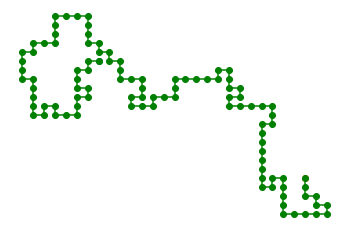
\includegraphics[width=\textwidth]{../images/loose_conf.png}
        \caption{глобула}
    \end{subfigure}
    \begin{subfigure}{0.45\textwidth}
	    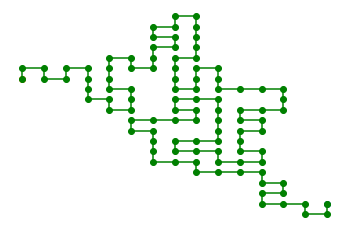
\includegraphics[width=\textwidth]{../images/dense_conf.png}
        \caption{клубок}
    \end{subfigure} 
	\caption{Примеры конформаций}
    \label{fig::globule_coil_example}
\end{figure}

Модели Изинга и модель конформаций представляют для нас интерес из-за геометрических свойств конформаций и известных свойств модели Изинга на различных решётках. А именно: точное решение для модели Изинга \cite{ising_solutions} показывает, что на одномерной сетке модель Изинга не имеет магнитного фазового перехода -- одномерная модель не становится магнитной ни при каких температурах, кроме абсолютного нуля. В то время как на двумерной сетке есть фазовый переход \cite{SAW_polymer_critical}, и она становится магнитной при низких температурах. Конформации так же имеют фазовый переход. Состояния конформаций называются глобулой или клубком и соответствуют низким и высоким температурам. Пример конформаций представлен на Рис. \ref{fig::globule_coil_example}. Структурно состояния конформации, которые в основном проявляются в глобулах и клубках, подобны одномерным и двумерным сеткам соответственно. Например количество соседей у вершин в глобулярных конформациях в основном 4 или 3, а в клубках у большинства вершин 2 соседа. Учитывая структурную схожесть фаз конформаций и решёток, можно предположить и магнитную схожесть.

Цель данной работы -- определить магнитные свойства конформаций в фазах глобула и клубок, сравнить свойства с двумерной и одномерной решёткой, определить точку фазового магнитного перехода в глобулах, если он существует, исследовать поведение магнитной модели вблизи геометрического перехода.